\subsection*{Explicación}
Un T-flip-flop hace lo mismo que un T-latch excepto que lo realiza en los posedge del clock.

\subsection*{Tabla de verdad}
\begin{figure}[h]
    \centering
    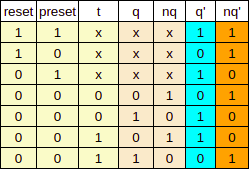
\includegraphics{fotos/TruthTable/arki-lab2-TT_tflipflop.png}
\end{figure}
%\subsection*{Mapa de Karnaugh}

%\subsection*{Ecuaciones booleanas}

%\subsection*{Resultados}
%\begin{figure}[h]
%    \centering
%    
%\end{figure}